\documentclass{article}%
\usepackage[T1]{fontenc}%
\usepackage[utf8]{inputenc}%
\usepackage{lmodern}%
\usepackage{textcomp}%
\usepackage{lastpage}%
\usepackage[head=40pt,margin=0.5in,bottom=0.6in]{geometry}%
\usepackage{graphicx}%
%
\title{\textbf{Exigen atención de servicios públicos a la alcaldía de Barinas}}%
\author{WALTER OBREGON}%
\date{24/09/2018}%
%
\begin{document}%
\normalsize%
\maketitle%
\textbf{URL: }%
http://www.eluniversal.com/venezuela/21497/exigen{-}atencion{-}de{-}servicios{-}publicos{-}a{-}la{-}alcaldia{-}de{-}barinas\newline%
%
\textbf{Periodico: }%
EU, %
ID: %
21497, %
Seccion: %
venezuela\newline%
%
\textbf{Palabras Claves: }%
NO\_TIENE\newline%
%
\textbf{Derecho: }%
2.8, %
Otros Derechos: %
3.2, %
Sub Derechos: %
2.8.1, 3.2.1\newline%
%
\textbf{EP: }%
NO\newline%
\newline%
%
\textbf{\textit{El dirigente de Acción Democrática,  Edgar Reyes, considera que la falta de interés de las autoridades ha llevado al colapso de las comunidades}}%
\newline%
\newline%
%
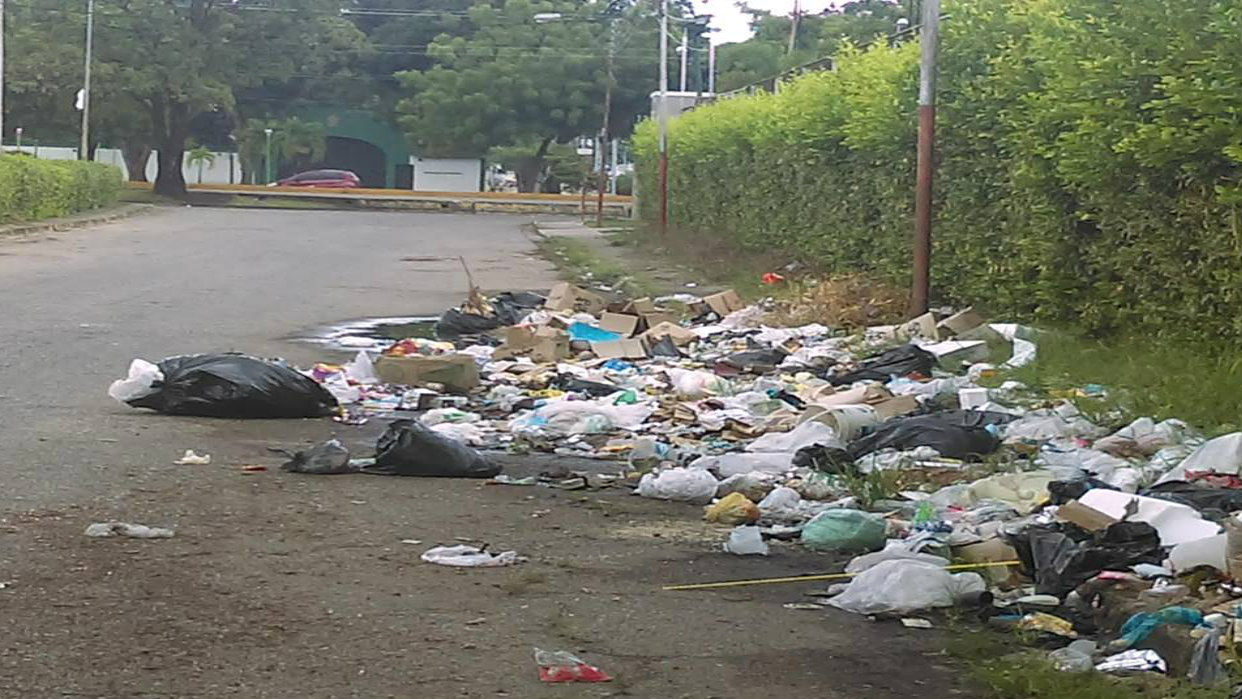
\includegraphics[width=300px]{196.jpg}%
\newline%
%
Barinas.{-} Fallas eléctricas, falta de agua y poca recolección de basura, son las principales demandas de servicios públicos que exigen a la alcaldía de Barinas, que para el dirigente municipal de Acción Democrática (AD), Edgar Reyes, es una instancia de Gobierno que se ha convertido en “un peso muerto para la ciudadanía”.%
\newline%
%
“Desde que Nancy Pérez asumió el poder en el municipio Barinas (diciembre de 2017), no hemos podido ver muestras de capacidad para solventar los problemas que aquejan a las comunidades, en materia de servicios públicos”, dijo Reyes.%
\newline%
%
El dirigente adeco considera que el reflejo del gobierno municipal está en los caños y desagües enmontados y llenos de desperdicios, también en el ornato y aseo de Barinas, en plazas y parques abandonados, junto al deterioro de los mercados.%
\newline%
%
Destacó que “en el cementerio municipal se ha instalado una mafia que cobra vacuna para sepultar, es algo nunca antes visto en Barinas bajo la mirada complaciente de la policía, Zodi y demás autoridades”.%
\newline%
%
Reyes hizo referencia a la desaparición de los programas sociales y de atención de las comunidades, como por ejemplo, el de salud en la calle, y denunció que los operativos de fiscalización representan un ataque sistemático al comercio, más el caos del tránsito ocasionado por la falta de semáforos en funcionamiento.%
\newline%
%
Calificó la gestión de la alcaldesa Nancy Pérez como "la peor en la historia municipal de Barinas", y agregó que “quizás se pudiese pensar que es una estrategia para la eliminación de esta instancia, debido al odio visceral que ha tenido el Gobierno en contra del proceso es descentralizado”.%
\newline%
%
Cree que no hay manera de poner excusas por la ineficiencia, porque la alcaldesa Pérez cuenta con el Gobierno nacional, con el presidente de la República, Nicolás Maduro y con la gobernación de Barinas en manos de Argenis Chávez.%
\newline%
%
\end{document}